\documentclass{a0poster}

\newcommand{\vphi}{\vec{\varphi}}
\newcommand{\vi}{{\vec{i}}}
\newcommand{\vj}{{\vec{j}}}
\newcommand{\vmu}{\vec{\mu}}

\usepackage{tikzposter}

\usetikzlibrary{positioning}
\usetikzlibrary{calc}
\usetikzlibrary{arrows,shapes,backgrounds}
\usetikzlibrary{shadows}

\renewcommand{\margin}{2}
% \renewcommand{\blockspacing}{2}
% \renewcommand{\blocktitlehight}{3}
% \renewcommand{\colnumber}{3}
% \renewcommand{\authorshift}{10}

\definecolor{colorone}{HTML}{006633} % default 116699
\definecolor{colortwo}{HTML}{DDFF99} % default CCCCCC
% \definecolor{colorthree}{HTML}{991111} % default 991111

% size of the document
\usepackage[margin=\margin cm, paperwidth=84.1cm, paperheight=118.9cm]{geometry}

% changing the fonts
\usepackage{cmbright}
\usepackage[light,math]{kurier}%iwona}
\usepackage[T1]{fontenc}

% add your packages here
\usepackage{hyperref}
\usepackage{listings}
\usepackage{bold-extra}

\lstdefinelanguage
  [GCC]{C++}
  []{C++}
{
  morekeywords={[2]__attribute__},%
  morekeywords={[3]vector_size,vec_t,uvec_t,fvec_t}%
}

\lstset{
  language={[GCC]C++},%
  basicstyle=\small\ttfamily,%
  keywordstyle=\color{blue}\ttfamily\bfseries,%
  keywordstyle=[2]\bfseries\color{darkgray},%
  keywordstyle=[3]\itshape,%
  commentstyle=\color{gray},%
  stringstyle=\color{green},%
% numbers=left,%
% numberstyle=\tiny,%
  stepnumber=1,%
  numbersep=5pt,%
% backgroundcolor=\color{lightlightgray},%
% frame=single,%
% rulecolor=\color{lightgray},%
% frameshape={RYRYNYYYY}{yny}{yny}{RYRYNYYYY},
  tabsize=2,%
  captionpos=b,%
  breaklines=true,%
  breakatwhitespace=false,%
  showspaces=false,%
  showtabs=false,%
  columns=flexible%
}

% \titlepic{}

\title{GPU-accelerated and CPU SIMD Optimized \\
Monte Carlo Simulation of $\phi^4$ Model}

\author{Piotr Bialas \and Jakub Kowal \and Adam Strzelecki \\
Faculty of Physics, Astronomy and Applied Computer Science \\
Jagiellonian University \\
ul. Reymonta 4, 30-059 Krakow, Poland \\
\\
\texttt{www.uj.edu.pl/web/zaklad-technologii-gier}
}

% defined in tikzposter, but now we want to include logo
\renewcommand{\titleblock}[2][($0.5*(0,\paperheight)-(0,\margin)$)]{%
\node[draw,frame,color=colortwo,fill=white,anchor=north,text=black] (title) at #1
   {
    \begin{minipage}{1cm}
      
\includegraphics{./UJ-logo.pdf}
    \end{minipage}
    \begin{minipage}{#2 cm}
      \maketitle
    \end{minipage}
  };
}

%%%%%%%%%%%%%%%%%%%%%%%%%%%%%%%%%%%%%%%%%%%%%%%%%%%%%%%%%%%%%%%%%%%%%%%%%%%%%%

\begin{document}
\AddToShipoutPicture{\BackgroundPicture}

\noindent % to have the picture right in the center
\begin{tikzpicture}
\initializesizeandshifts
\titleblock{50}

\begin{blocknode}[($(title.south)-(xshift)-(yshift)$)]{Introduction}

This contribution is concerned with an efficient implementation of the
Monte-Carlo simulations of the $\varphi^4$ model\cite{parisi}. The problem is
defined as follows: having a vector field $\vphi$ defined on a regular
rectangular two or three dimensional grid we want to generate the field
configurations with probability proportional to $\exp(-H(\vphi))$ where
$H(\vphi)$ is some function of all the fields $\vphi_i$. \\

The actual generation is done by the mean of the Metropolis algorithm. This
amounts to sequentially updating all the points of the lattice. The crucial
feature of this algorithm is that the update is local {\em i.e.} the new value
of the field in a given point depends only on the values of fields in the
immediate neighborhood of the updated point. In our case this neighborhood is
extended compared to usual nearest neighbors. The update is random and requires
a good source of pseudo-random numbers. We use the Tausworthe
RNG\cite{howes_thomas07}.

\end{blocknode}

%%%%%%%%%%%%%%%%%%%%%%%%%%%%%%%%%%%%%%%%%%%%%%%%%%%%%%%%%%%%%%%%%%%%%%%%%%%%%%

\begin{blocknode}{Parallelization}

While model is inherently parallelizable, grid points that lie in the same
neighborhood cannot be updated together. Taking into account a larger
neighborhood means that a simple checkerboard decomposition pattern cannot be
used and we have devised a new grid decomposition scheme. \\

\begin{center}

\begin{tikzpicture}[scale=1.9]

\draw[very thin, gray] (-.5,-.5) grid (15.5,15.5);

\foreach \x in {0,4,...,12}
  \foreach \y in {0,4,...,12} {
    \pgfmathtruncatemacro\n{Mod(\x/4,2)+2*Mod(\y/4,2)+1}
    \draw[colorone, xshift=\x cm, yshift=\y cm, rounded corners=2pt]
      (-.4,-.4) rectangle node[red, fill opacity=.5, anchor=center, font=\Huge\bfseries\sffamily] {\n} (3.4,3.4);
  }

\foreach \x in {0,...,15}
  \foreach \y in {0,...,15}
    \path[draw=black,fill=white] (\x, \y) circle(.25);

\foreach \x in {4,...,7}
  \foreach \y in {4,...,7}
    \fill[black] (\x, \y) circle(.25);

\foreach \x in {4,...,7}
  \foreach \y in {2,3,8,9} {
    \fill[gray] (\x,\y) circle(.25);
    \fill[gray] (\y,\x) circle(.25);
  }

\foreach \p in {(3,3),(3,8),(8,3),(8,8)}
  \fill[gray] \p circle(.25);

\end{tikzpicture}

\end{center}

\textbf{Figure 1} The partition of the lattice into blocks. The blocks with same
number are processed in parallel by different thread blocks. \\
\vspace{2cm}

\begin{center}

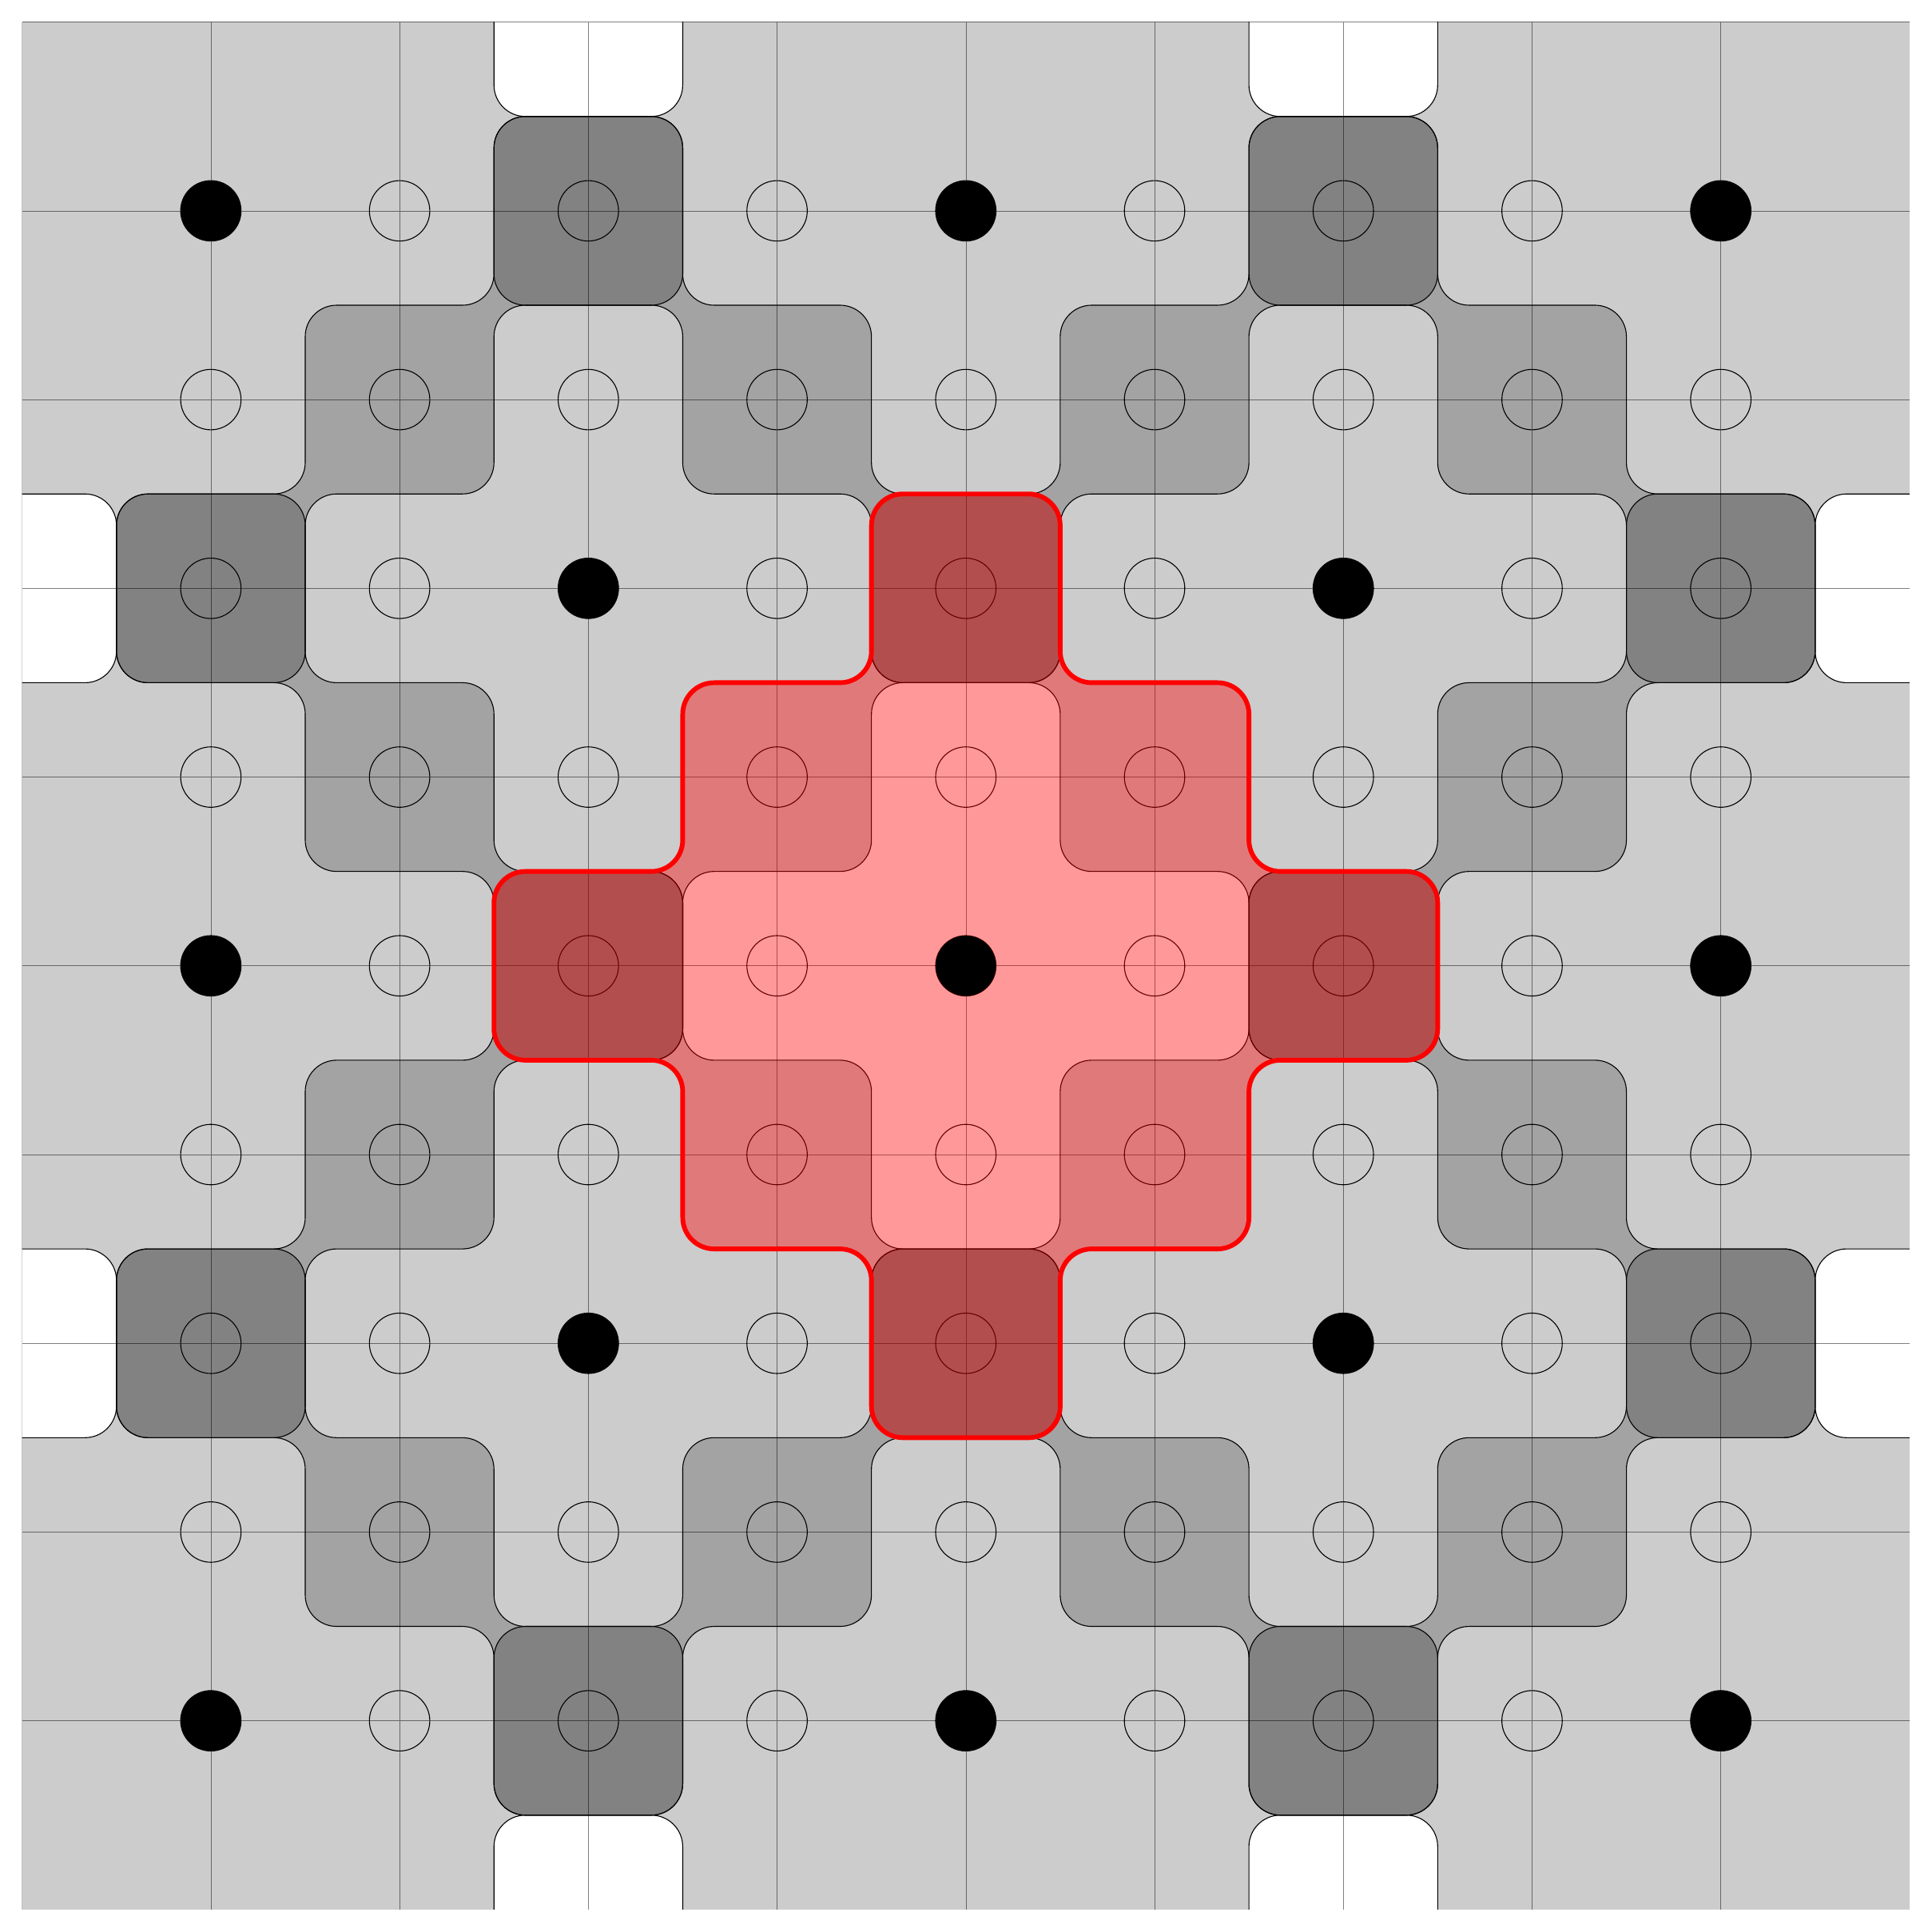
\begin{tikzpicture}[scale=3]

\clip[rounded corners=0cm] (-3,-3) rectangle (7,7);

\draw[help lines] (-3.0,-3.0) grid (7.0,7.0);

% lattice points
\foreach \x in {-2,-1,0,1,2,3,4,5,6}
  \foreach \y in {-2,-1,0,1,2,3,4,5,6}
    \draw (\x,\y) + (.0,.0) circle (.16);

% neighborhood
\def\neighborhood{--
  ++(0,-.5)-- ++(1,0)-- ++(0,-.5)-- ++(0,-.5)-- ++(1,0)--
  ++(0,-1.0)-- ++(1,0)-- ++(0,1.0)-- ++(1,0)-- ++(0,1.0)-- ++(1,0)--
  ++(0,1)-- ++(-1,0)-- ++(0,1)-- ++(-1,0)-- ++(0,1)-- ++(-1,0)-- ++(0,-1)--
  ++(-1,0)-- ++(0,-1)-- ++(-1,0)-- ++(0,-.6)}

\foreach \p in {(-2.5,4.0),(1.5,4.0),
                (-2.5,.0),(1.5,.0),
                (-4.5,2.0),(3.5,2.0),
                (-4.5,6.0),(-.5,6.0),(3.5,6.0),
                (-4.5,-2.0),(-.5,-2.0),(3.5,-2.0)}
  \path[draw=black,fill,fill opacity=.2,rounded corners=.5cm,shorten >=2pt]
    \p \neighborhood;

% main center neighborhood

\path[draw=red,fill=red,fill opacity=.4,rounded corners=.5cm,shorten >=2pt,line width=.75mm,cap=round,join=round] (-.5,2.0) \neighborhood;

\foreach \p in {
  (-2, 2),( 2, 2),( 6, 2),
  ( 0, 4),( 0, 0),( 4, 0),( 4, 4),
  (-2,-2),( 2,-2),( 6,-2),
  (-2, 6),( 2, 6),( 6, 6)}
  \fill[black] \p circle(.16);

\end{tikzpicture}

\end{center}

\textbf{Figure 2} Partitioning of the blocks into disjoint sublattices. Thick
black line denotes the neighborhood used in updating the center point. Black
points are processes in parallel by different threads of the same thread block.

\end{blocknode}

%%%%%%%%%%%%%%%%%%%%%%%%%%%%%%%%%%%%%%%%%%%%%%%%%%%%%%%%%%%%%%%%%%%%%%%%%%%%%%

\begin{blocknode}[($(title.south)+(xshift)-(yshift)$)]{Tausworthe RNG}

\lstinputlisting{MC3-tausworthe.cpp}

\end{blocknode}

%%%%%%%%%%%%%%%%%%%%%%%%%%%%%%%%%%%%%%%%%%%%%%%%%%%%%%%%%%%%%%%%%%%%%%%%%%%%%%

\begin{blocknode}{GPU Implementation}

On GPU we adopt the hierarchical scheme from ref.~\cite{weigel} suitably
modified to account for bigger neighborhood. We first divide the whole lattice
in blocks of $32\times 32$ points. Then we start a kernel that process every
forth block. Each block is assigned to a block of 128 threads. First we fetch
the values of the fields from global to shared memory (including border
points). After that each thread updates one point from the first partition.
Then after synchronization, next partition is updated and so on. After
processing all eight(2D) or 16 (3D) partitions the kernel writes the shared
memory back into global and new kernel is started processing next batch of
blocks. Altogether in this way we managed to achieve $0.13$ nanoseconds for
single lattice field update on \emph{NVIDIA GTX 470}, reaching around $430$
Gflops that is $40\%$ of $1088$ Gflops peak performance of this device.

\end{blocknode}

%%%%%%%%%%%%%%%%%%%%%%%%%%%%%%%%%%%%%%%%%%%%%%%%%%%%%%%%%%%%%%%%%%%%%%%%%%%%%%

\begin{blocknode}{CPU Implementation}

In order to provide unbiased CPU vs GPU speed up results we provide
multithreaded vectorized CPU implementation. It uses OpenMP for parallel
execution, SSE/AVX and compiler vector extensions for vectorization. This
implementation does mimic GPU SIMT execution model. The SIMD instructions are
used to process four (SSE) or eight (AVX) updates in parallel. We use
partitions as on GPU but we use only one level {\em i.e.} we do not partition
the lattice into blocks. However not all scalar \emph{x86} instructions have
vector counterparts. In particular direct \emph{XMM} registers gather and
scatter and vectorized integer operations for full length AVX 256-bit registers
are missing, which makes impossible to port random number generator from
128-bit SSE to 256-bit AVX. Initially planned for AVX standard, these were
postponed to AVX2 planned for 2013. As soon AVX2 capable CPU devices appear on
the market we plan to revise our evaluation.

\end{blocknode}

%%%%%%%%%%%%%%%%%%%%%%%%%%%%%%%%%%%%%%%%%%%%%%%%%%%%%%%%%%%%%%%%%%%%%%%%%%%%%%

\begin{blocknode}{Conclusions}

Our CPU \emph{OpenMP} and \emph{SSE/AVX} implementation compiled via GCC 4.4 or
higher and running on \emph{Intel Core i5 2.5 Ghz} quad core CPU presented
$15\times$ performance boost comparing to single threaded scalar code and
$3.76$ nanoseconds for single lattice field update. Which gives the $15$ Gflops
that is $\sim10\%$ of the $160$ Gflops peak performance of tested i5 CPU. There
is no significant increase in performance while switching from SSE to AVX
instructions. \\

\innerblock{Benchmark Results}{
\begin{center}
\huge \textbf{GPU} $0.13$ ns/update \ \textbf{CPU} \huge $3.76$ ns/update
\end{center}}

This gives around $28\times$ advantage to GPU, which is noticeably less than
promised by many publications, however much higher that comes from comparison
of tested i5 CPU to \emph{GTX 470}. This can be traced back to 128-bit only
\emph{Tausworthe} random number generator implementation and inefficient vector
store and load operations (gather/scatter).

\end{blocknode}

%%%%%%%%%%%%%%%%%%%%%%%%%%%%%%%%%%%%%%%%%%%%%%%%%%%%%%%%%%%%%%%%%%%%%%%%%%%%%%

\begin{blocknode}{References}

\renewcommand{\section}[2]{}
\begin{thebibliography}{9}
\bibitem{parisi} G.~Parisi ``Statistical Field Theory'' Chapter 5, Perseus Books Publishing (1998).
\bibitem{weigel} M.~Weigel, J. Comput. Phys. \textbf{231}, 3064 (2012).
\bibitem{howes_thomas07}
Lee Howes and David Thomas.
``{\em Efficient random number generation and application using {CUDA}.}''
In Hubert Nguyen, editor, {\em GPU Gems 3}, chapter~37. Addison
  Wesley, August 2007.
\end{thebibliography}

\end{blocknode}

\end{tikzpicture}

\end{document}
